% !TEX TS-program = pdflatex
% !TEX encoding = UTF-8 Unicode

% This is a simple template for a LaTeX document using the "article" class.
% See "book", "report", "letter" for other types of document.

\documentclass[11pt]{article} % use larger type; default would be 10pt

\usepackage[utf8]{inputenc} % set input encoding (not needed with XeLaTeX)

%%% Examples of Article customizations
% These packages are optional, depending whether you want the features they provide.
% See the LaTeX Companion or other references for full information.

%%% PAGE DIMENSIONS
\usepackage{geometry} % to change the page dimensions
\geometry{a4paper} % or letterpaper (US) or a5paper or....
% \geometry{margin=2in} % for example, change the margins to 2 inches all round
% \geometry{landscape} % set up the page for landscape
%   read geometry.pdf for detailed page layout information

\usepackage{graphicx} % support the \includegraphics command and options

% \usepackage[parfill]{parskip} % Activate to begin paragraphs with an empty line rather than an indent

%%% PACKAGES
\usepackage{booktabs} % for much better looking tables
\usepackage{array} % for better arrays (eg matrices) in maths
\usepackage{paralist} % very flexible & customisable lists (eg. enumerate/itemize, etc.)
\usepackage{verbatim} % adds environment for commenting out blocks of text & for better verbatim
\usepackage{subfig} % make it possible to include more than one captioned figure/table in a single float
% These packages are all incorporated in the memoir class to one degree or another...

%%% HEADERS & FOOTERS
\usepackage{fancyhdr} % This should be set AFTER setting up the page geometry
%\pagestyle{fancy} % options: empty , plain , fancy
\renewcommand{\headrulewidth}{0pt} % customise the layout...
\lhead{}\chead{}\rhead{}
\lfoot{}\cfoot{\thepage}\rfoot{}

%%% SECTION TITLE APPEARANCE
\usepackage{sectsty}
%\allsectionsfont{\sffamily\mdseries\upshape} % (See the fntguide.pdf for font help)
% (This matches ConTeXt defaults)

%%% ToC (table of contents) APPEARANCE
\usepackage[nottoc,notlof,notlot]{tocbibind} % Put the bibliography in the ToC
\usepackage[titles,subfigure]{tocloft} % Alter the style of the Table of Contents
\renewcommand{\cftsecfont}{\rmfamily\mdseries\upshape}
\renewcommand{\cftsecpagefont}{\rmfamily\mdseries\upshape} % No bold!

%%% END Article customizations

%%% The "real" document content comes below...

\title{Design Principles and Methods - Odometry Lab Report}
\author{Harley Wiltzer (260690006)\\Juliette Regimbal (260657238)}
\date{October 6, 2016} % Activate to display a given date or no date (if empty),
         % otherwise the current date is printed 
\pagenumbering{gobble}
\begin{document}
\maketitle

\section{Objective}
To determine the accuracy of the implemented odometry system, and implement a simple correction using a light sensor.
\section{Method}
\begin{enumerate}
\item In the file \texttt{Odometer.java}, implement code that performs the task of an odometer as
described in the Odometry tutorial and in class. You should only need to add member variables
to and modify the \texttt{run()} method of the /texttt{Odometer} class.
\item Run the robot in a 3-by-3 tile square (where one tile is 30.48 cm in linear dimension) using the
provided code and tweak the \texttt{leftRadius}, \texttt{rightRadius}, and \texttt{width} parameters passed
to the \texttt{SquareDriver.drive()} method in \texttt{Lab2.java} until the robot returns
(approximately) to its starting position. If your left and right wheel motors are not connected to
motor ports A and B respectively, you may need to also modify those parameters. The call to
\texttt{SquareDriver.drive()} is shown below.\\
\\
\texttt{SquareDriver.drive(leftMotor, rightMotor, leftRadius, rightRadius, width);}
\item Now, run the robot in a 3-by-3 tile square ten (10) times and measure the signed x and ydistances from the actual location of the robot on the field (recalling that its starting position isthe origin) to that reported by its odometer. Feel free to calibrate your odometer prior to thisstep. Record these results. (Note: Your odometer is reporting the position of the point directlybetween your wheel axles).
\item In the file \texttt{OdometryCorrection.java}, implement code that, using the light sensor,detects grid lines and updates/corrects the odometer's position data as needed. Your robotshould start its motion in the center of a tile, and thus grid lines will occur at x = 15 cm, 45 cm,75 cm, ... and y = 15 cm, 45 cm, 75 cm, .... You do not need to account for grid line intersectionsin this case.
\item Repeat step (3) with your odometry correction enabled. Do not recalibrate your odometer.
\item Demonstrate to a TA your code. The TA will first 'float' your motors (i.e. the motors will be shut off in such a way that they do not provide resistance to being backdriven) and push your robot on the field to confirm that your odometer works correctly. The TA will then start your robot off-center in a tile and look for it to report its correct position after running in a 3-by-3 tile square.
\end{enumerate}
\section{Data}
\begin{center}
\begin{tabular}{ | c | c | c | c | }
\multicolumn{4}{c}{Offset from Origin - Correction Disabled} \\ \hline
Trial No. & X (cm) & Y (cm) & $\theta$ (rad)\\ \hline
1 & -0.42 & -0.66 & 0.01 \\ \hline
2 & -0.67 & -0.86 & 0.01 \\ \hline
3 & -0.84 & -0.84 & 0.01 \\ \hline
4 & -0.45 & -0.46 & 0.01 \\ \hline
5 & -0.64 & -0.82 & 0.01 \\ \hline
6 & -0.82 & -0.45 & 0.01 \\ \hline
7 & -0.69 & -0.66 & 0.01 \\ \hline
8 & -0.39 & -0.44 & 0.01 \\ \hline
9 & -0.84 & -0.66 & 0.01 \\ \hline
10 & -0.64 & -0.63 & 0.01 \\ \hline
Standard Deviation & 0.17 & 0.16 & \\ \hline
\end{tabular}
\end{center}

\begin{center}
\begin{tabular}{ | c | c | c | c | }
\multicolumn{4}{c}{Offset from Origin - Correction Enabled} \\ \hline
Trial No. & X (cm) & Y (cm) & $\theta$ (rad)\\ \hline
1 & -0.04 & -0.09 & 0.01 \\ \hline
2 & -0.28 & -0.18 & 0.01 \\ \hline
3 & -0.18 & -0.19 & 0.01 \\ \hline
4 & -0.28 & -0.27 & 0.01 \\ \hline
5 & -0.31 & -0.18 & 0.01 \\ \hline
6 & -0.19 & -0.20 & 0.01 \\ \hline
7 & -0.27 & -0.13 & 0.01 \\ \hline
8 & -0.18 & -0.25 & 0.01 \\ \hline
9 & -0.08 & -0.12 & 0.01 \\ \hline
10 & -0.17 & -0.11 & 0.01 \\ \hline
Standard Deviation & 0.09 & 0.06 & \\ \hline
\end{tabular}
\end{center}

\section{Data Analysis}
\subsection{What was the standard deviation of the results without correction? Did it decrease when
the correction was introduced? Explain why/why not.}
The standard deviation of the data corresponding to the robot's distance from the origin without any
odometry correction was 0.17cm on the X axis and 0.16cm on the Y axis. The standard deviation did
decrease significantly with the odometry correction enabled, as the standard deviation of the X
position was measured to be 0.09cm, and only 0.06cm for the Y position. This makes sense, as the
odometer reading was modified when the robot passed a grid line. The grid lines are a known, fixed
distance away from each other, thus change in position can be accurately measured (in one spatial
axis at a time) by detecting the grid lines. Therefore, with the odometry correction, no matter how
much the wheels spin the robot could more accurately report its position as it crosses the gridline,
reducing the effect of wheel spin on the overall odometer reading. This allows for more precise
measurements.
\subsection{With correction, do you expect that the error in the x position or the y position will
be smaller? Explain.}
With the odometry correction, the errors in the x position and y position should be smaller, as
described in \textbf{4.1}. Considering the design implemented in this lab, there is no reason why
one direction would see more error than the other, as the motion is perfectly symmetric. To avoid
direction bias and compromised corrections to the odometer readings, the \texttt{OdometryCorrection}
implementation does not tamper with odometer data at the first line crossing after each corner.
Unmeasurable slipping occurs when turning corners, thus there is no guarantee in displacement when
the robot turns a corner and crosses a line. Therefore, \texttt{OdometryCorrection} simply saves the
current odometer readings at the first line crossing after a corner, and offsets those readings at
subsequent line crossings. This way, there is no reason why either the x position or y position
should have smaller error.
%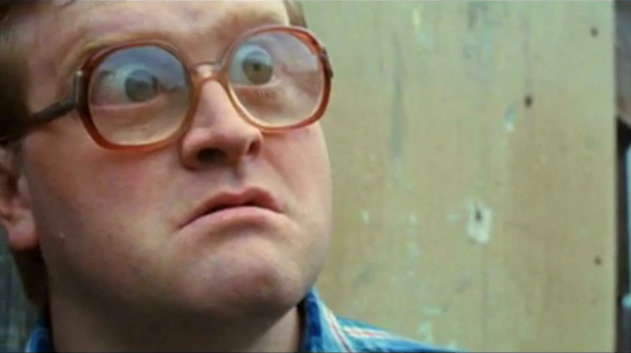
\includegraphics{Bubbles.png}
\section{Observations and Conclusion}

\section{Further Improvements}
\subsection{Propose a means of, in software, reducing the slip of the robot's wheels (do not provide code).}
To reduce the slip of the robot's wheels in software, the acceleration of the motors can be
decreased. When the angular acceleration of a wheel is too high, slipping occurs. The motors of the
robot accelerate when the robot starts moving and when it turns corners. Thus, by reducing
the acceleration of the motors, the amount of slipping can be drastically reduced.
\subsection{Propose a means of, in software, correcting the angle reported by the odometer, when (do not provide code):}
\subsubsection{The robot has two light sensors.}
Say the robot has two light sensors at its front, one on each side. When one sensor detects a grid
line, the current odometer reading of position is stored. Then, when the other sensor
detects a grid line, the new position readings are compared to the saved ones to determine the
change in tachometer readings of the left and right motors. With this data, the angle can be
calculated.
\subsubsection{The robot has only one light sensor.}
With one light sensor, the angle of the robot can be corrected as well. At each line crossing, the
odometer reading of the robot can be stored. For the purpose of explanation, assume the robot is
moving in the positive y direction. Now, between two line crossings, it is guaranteed that the y
position of the robot has increased by 30.48cm. The difference in x positions can be measured then,
and the angle $\theta$ can be calculated as $\theta = \arctan{(\frac{\Delta x}{30.48})}$.

\end{document}
